\chapter{Risultati}
\label{chap:cap4}
Lo scopo principale e, se vogliamo la sfida, di ogni problema di ML consiste nell'ottenere delle buone \textit{performance} dell'algoritmo su dati nuovi e mai visti. Come descritto nel capitolo precedente, dopo aver scelto il miglior modello di albero decisionale mediante la tecnica del \textit{pruning}, bisogna valutare le sue prestazioni sul \textit{test set}. In questo Capitolo, dunque, vengono presentati i risultati ottenuti dal classificatore su ognuno dei \textit{dataset} considerati. Gli strumenti utilizzati per la valutazione sono le matrici di confusione (Sez. \ref{subsec:confmatr}) e le metriche di precisione, richiamo ed \textit{F-score}. Infine, proprio grazie alle caratteristiche degli alberi decisionali, è possibile fornire un'interpretazione dei risultati sulla base dell'\textit{importanza} delle \textit{features}.

\section{Valutazione delle performance}
Sono stati utilizzati sei \textit{dataset} diversi per la previsione della presenza di IMBHs al centro di GCs a partire dalle caratteristiche dinamiche delle MSPs che si trovano nelle regioni centrali degli ammassi. I \textit{dataset} differiscono tra loro per il numero di MSPs selezionate casualmente in queste zone per ogni ammasso: 1, 5, 10, 20, 30 o 40.

Le prestazioni degli alberi decisionali vengono valutate sui relativi \textit{test set} in base alla loro capacità nel classificare gli ammassi nella \textbf{classe 0} o nella \textbf{classe 1}.\\
In figura \ref{fig:risultati_matrici} sono riportate le matrici di confusione ottenute considerando il miglior modello classificatore per ogni \textit{dataset}. Esse sono un utile strumento per visualizzare la qualità delle classificazioni. Infatti, mettono in relazione quelli che sono i reali valori delle \textit{labels} (\textit{"True label"}) con i valori che, invece, sono stati predetti (\textit{"Predicted label"}) per ciascuna classe. Nelle celle sulle diagonali vi è il numero di risposte corrette date dal classificatore, mentre nelle altre celle vi è il numero di risposte sbagliate. Si vede che, con l'aumentare del numero di MSPs selezionate nel centro di ciascun ammasso, aumenta anche il numero di risposte corrette da parte dell'albero decisionale. In particolare, i corrispondenti valori delle metriche di precisione, richiamo ed \textit{F-score} sono riportati nelle tabelle \ref{tab:risultati_metriche}.
Per maggiore chiarezza, infine, in figura \ref{fig:f1_num}, vi è l'andamento della \textit{F-score} per ciascuna classe, in funzione del numero di MSPs considerato per ogni ammasso. Si vede che, per entrambe le classi, i valori di \textit{F-score} aumentano notevolmente (di circa il $10\%$) con l'aumentare del numero di MSPs, fino a 10 MSPs per ammasso. Da 20 MSPs in poi, le \textit{F-score} si stabilizzano al $72\%$ e $73\%$.\\
\textbf{Discussione: risultati buoni? perchè? perchè ad un certo punto la f1 si stabilizza?}

\begin{figure}[H]
\centering
\subfloat[1 MSP per ammasso.]{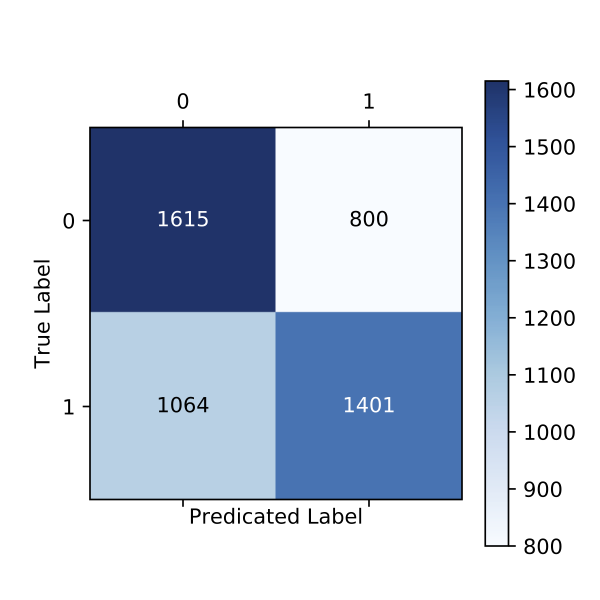
\includegraphics[width = 2in]{images/cm_1part.png}}
\qquad
\subfloat[5 MSPs per ammasso.]{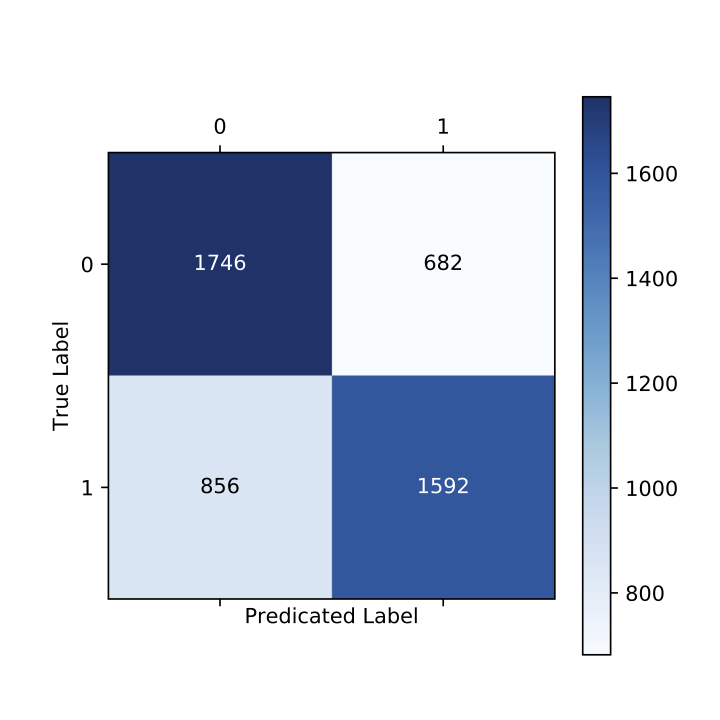
\includegraphics[width = 2in]{images/cm_5part.png}}\\
\subfloat[10 MSPs per ammasso.]{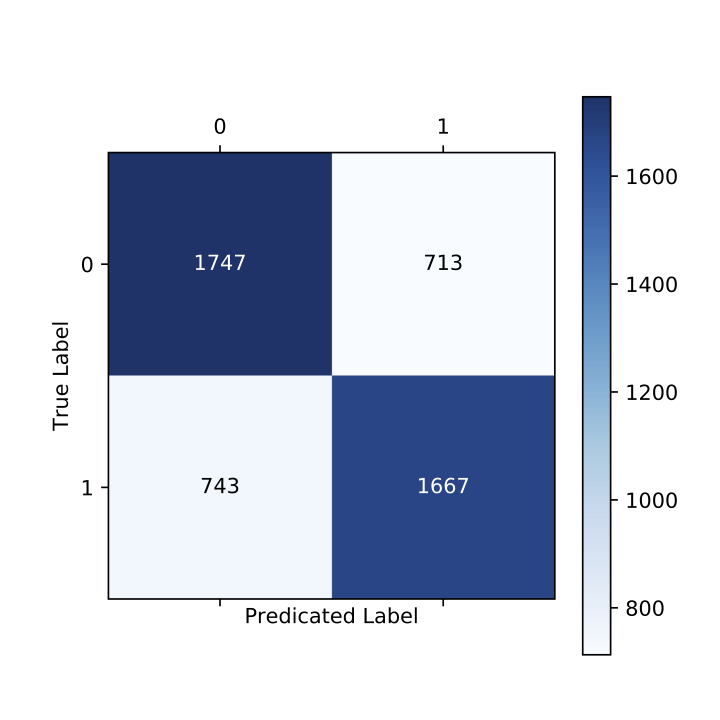
\includegraphics[width = 2in]{images/cm_10part.png}}
\qquad
\subfloat[20 MSPs per ammasso.]{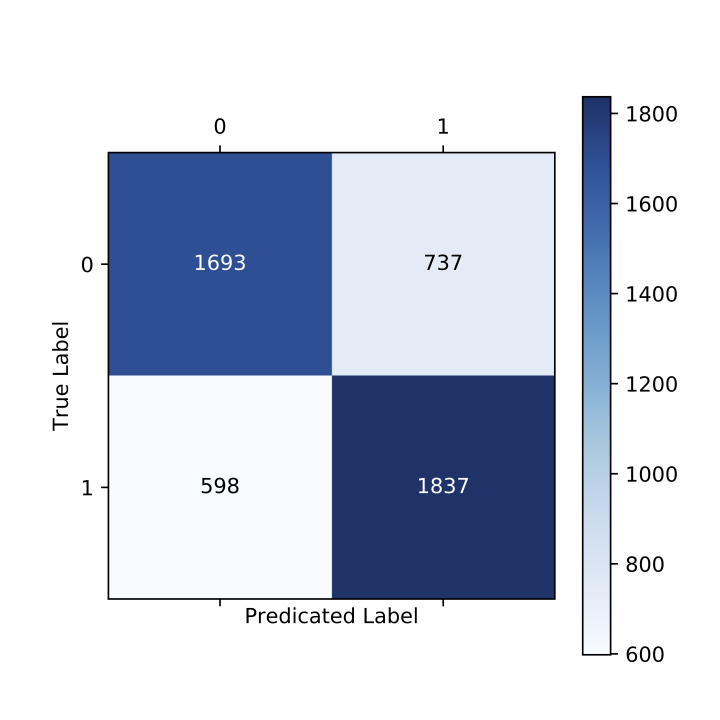
\includegraphics[width = 2in]{images/cm_20part.png}}\\
\subfloat[30 MSPs per ammasso.]{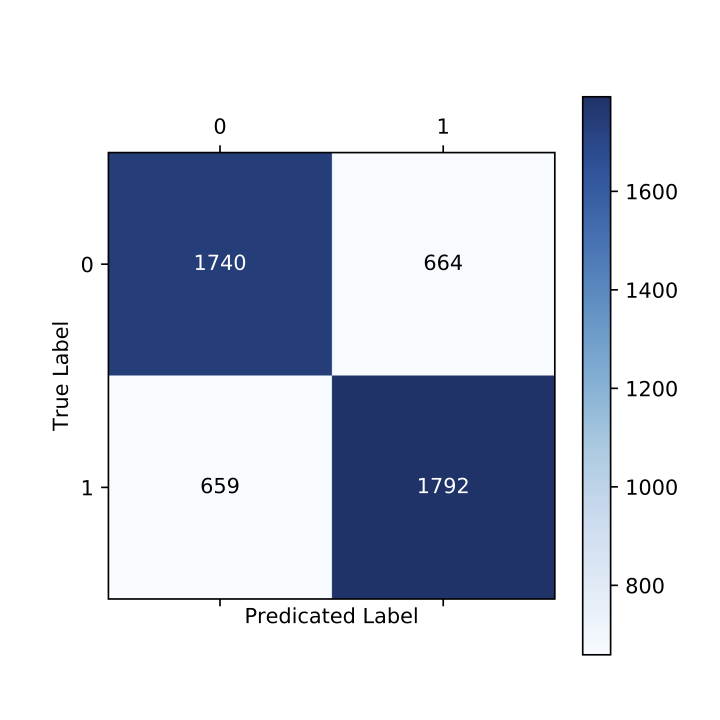
\includegraphics[width = 2in]{images/cm_30part.png}}
\qquad
\subfloat[40 MSPs per ammasso.]{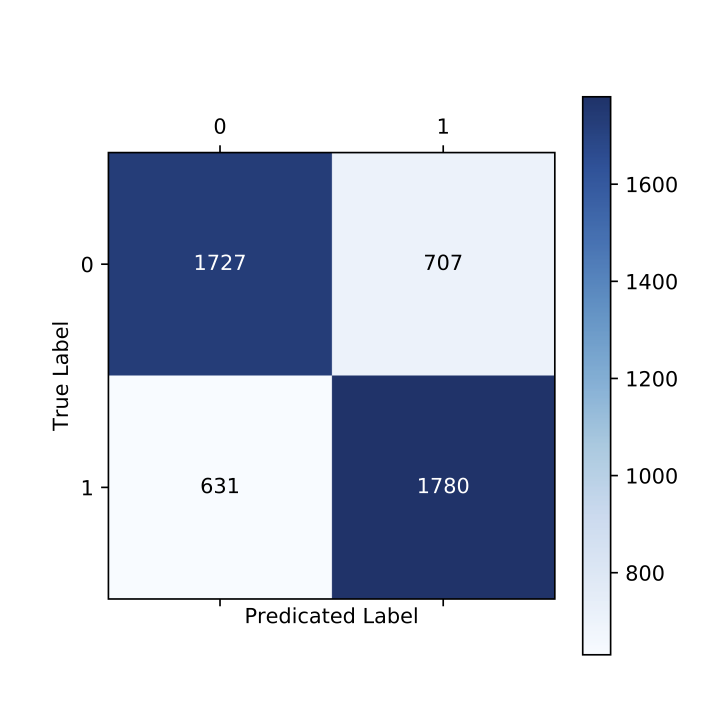
\includegraphics[width = 2in]{images/cm_40part.png}}
\caption{Matrici di confusione ottenute sui \textit{test set} per i sei diversi \textit{dataset}.}
\label{fig:risultati_matrici}
\end{figure}
\begin{table}[H]
\centering 
\subfloat[1 MSP per ammasso.]{%
	\begin{tabular}{cccc}\hline 
	classe & precisione & richiamo & F-score \\
	\hline
	0 & 0.60 & 0.67 & 0.63 \\
	\hline
	1 & 0.64 & 0.57 & 0.60\\
	\hline
	\end{tabular} 
	}
\qquad
\subfloat[5 MSPs per ammasso.]{%
	\begin{tabular}{cccc}\hline 
	classe & precisione & richiamo & F-score \\
	\hline
	0 & 0.67 & 0.72 & 0.69 \\
	\hline
	1 & 0.70 & 0.65 & 0.67\\
	\hline
	\end{tabular}} \\
\subfloat[10 MSPs per ammasso.]{%
	\begin{tabular}{cccc}\hline 
	classe & precisione & richiamo & F-score \\
	\hline
	0 & 0.70 & 0.71 & 0.71 \\
	\hline
	1 & 0.70 & 0.69 & 0.70\\
	\hline
	\end{tabular} 
		} 
\qquad
\subfloat[20 MSPs per ammasso.]{%
	\begin{tabular}{cccc}\hline 
	classe & precisione & richiamo & F-score \\
	\hline
	0 & 0.74 & 0.70 & 0.72  \\
	\hline
	1 & 0.71 & 0.75 & 0.73\\
	\hline
	\end{tabular}} \\
\subfloat[30 MSPs per ammasso.]{%
	\begin{tabular}{cccc}\hline 
	classe & precisione & richiamo & F-score \\
	\hline
	0 & 0.73 & 0.72 & 0.72 \\
	\hline
	1 & 0.73 & 0.73 & 0.73\\
	\hline
	\end{tabular} 
		}
\qquad
\subfloat[40 MSPs per ammasso.]{%
	\begin{tabular}{cccc}\hline 
	classe & precisione & richiamo & F-score \\
	\hline
	0 & 0.73 & 0.71 & 0.72 \\
	\hline
	1 & 0.72 & 0.74 & 0.73\\
	\hline
	\end{tabular}} \\
\caption{Risultati di precisione, richiamo ed F-score per ciascuna classe, ottenuti sui \textit{test set} per i sei diversi \textit{dataset}.} 
\label{tab:risultati_metriche}
\end{table}

\begin{figure}[H]
\begin{center}
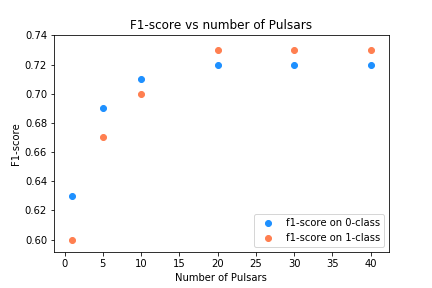
\includegraphics[width=1\columnwidth]{images/f1_num.png}
\end{center}
\caption{Andamento della \textit{F-score} per le due distinte classi in funzione del numero di MSPs considerate per ogni ammasso.}
\label{fig:f1_num}
\end{figure}

\section{Interprtazione dei risultati}
Gli alberi decisionali, soprattutto se non sono molto profondi, sono semplici da interpretare, in quanto essi possono essere visualizzati.\\
In figura \ref{fig:tree_1part} è riportato un esempio di albero decisionale ottenuto con il \textit{dataset} relativo ad una MSP estratta per ogni ammasso.

L'interpretazione è semplice: partendo dal nodo radice si percorre l'albero passando per i nodi successivi per mezzo dei rami. Questi ultimi suggeriscono quale sottoinsime andremo a guardare. Abbiamo già visto che gli \textit{split}, per ogni sottoinsieme, vengono decisi in base ad una misura di impurità fatta sulla valutazione dell'indice di Gini.\\ L'algoritmo sceglie come nodo radice quello con impurità più bassa, ossia quello con il valore di indice di Gini minore.\\ Una volta deciso il nodo radice, l’albero viene ingrandito ad una profondità pari ad uno. Lo stesso processo viene ripetuto per gli altri nodi nell’albero fino a raggiungere la massima profondità. In questo caso, stiamo interpretando un albero con profondità pari a 7, ottenuta in seguito alla fase di potatura.
\begin{figure}[H]
\begin{center}
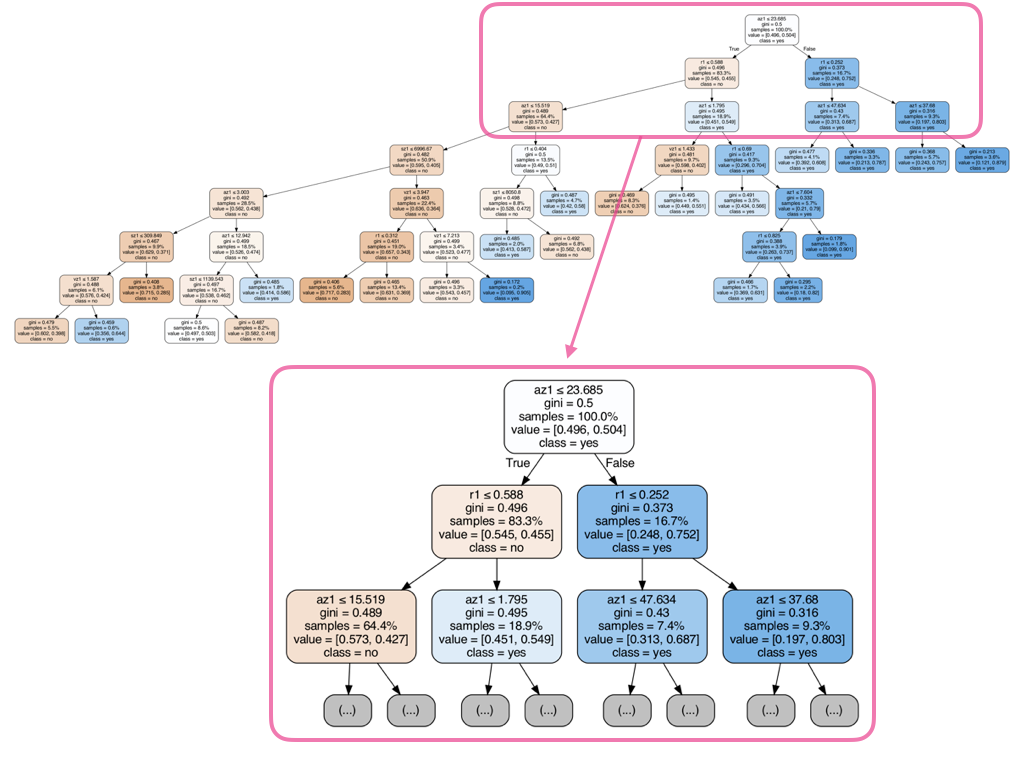
\includegraphics[width=1.1\columnwidth]{images/tree_1part_ok.png}
\end{center}
\caption{Un esempio di albero decisionale ottenuto a partire dal \textit{dataset} di 1 MSP selezionata nella regione centrale di ogni ammasso considerato. Per chiarezza è stato eseguito uno zoom nei primi \textit{split} dell'albero.}
\label{fig:tree_1part}
\end{figure}
Per maggior chiarezza, in figura \ref{fig:tree_1part} è stato fatto uno zoom sui primi \textit{split}, in particolare per il primo nodo abbiamo che:
\begin{itemize}
    \item $\mathbf{a_{z1} \le 23.685}$: il primo \textit{split} viene fatto sulla \textit{feature} $a_{z1}$, ovvero ci si chiede se essa è minore o uguale di 23.685 e, in base al risultato, si segue il percorso \textit{True} (freccia di sinistra) o \textit{False} (freccia di destra);
    \item $\mathbf{gini = 0.5}$: è l'indice di Gini per la \textit{feature} $a_{z1}$. Un valore dell'indice di Gini pari a 0 significa che il nodo è puro, ossia che esiste solo una classe (quindi che gli ammassi appartengono tutti alla \textbf{classe “yes”} o alla \textbf{classe “no”}). Al contrario, un valore maggiore di 0, come nel nodo radice, ci indica che i campioni all’interno del nodo appartengono ad entrambe le classi; 
    \item $\mathbf{samples = 100\%}$: indica la percentuale di ammassi da classificare appartenenti al \textit{training set}. Nel nodo radice è corretto aspettarsi che ancora tutti gli ammassi devono essere classificati;
    \item $\mathbf{value = [0.496, 0.504]}$: indica la frazione di ammassi di quel nodo che ricadono in ciascuna classe. Ciò significa che nel nodo radice il $49.6\%$ degli ammassi appartiene alla \textbf{classe "no"} (che abbiamo anche chiamato \textbf{classe 0}) ed il restante $50.4\%$ fa parte della \textbf{classe "yes"} (chiamata anche \textbf{classe 1});
    \item $\mathbf{class = yes}$: rappresenta la previsione su quel determinato nodo e si ricava da \textbf{value}. Infatti, dal punto sopra, capiamo che nel nodo c'è una percentuale maggiore di campioni appartenenti alla \textbf{classe “yes”}.
\end{itemize}
Queste denominazioni vengono ripetute per i vari nodi successivi dell’albero. Nello specifico, si può notare che la somma delle \textit{samples} dei nodi figli restituisce il valore \textit{samples} dei nodi padri.\\
Inoltre, la \textbf{classe "yes"} è identificata con l'azzurro, mentre la \textbf{classe "no"} con l'arancione. L'intensità della colorazione di ogni nodo varia in base all'accuratezza della previsione: vediamo che nei nodi di azzurro più intenso una percentuale maggiore di ammassi viene classificata in \textbf{"yes"} e in quelli di arancione più intenso, invece, una percentuale maggiore di ammassi viene classificata in \textbf{"no"}.\\
Infine, nei nodi foglia non appaiono più le \textit{features}, in quanto si è raggiunta la massima profondità e tutti gli ammassi in quel nodo, sono stati classificati.

In ultimo, è possibile valutare l'importanza delle diverse \textit{features} per un albero decisionale. L'importanza complessiva di una singola \textit{feature} può essere calcolata nel modo seguente: bisogna esaminare tutti gli \textit{split} per i quali la \textit{feature} è stata utilizzata e misurare quanto essa ha ridotto l'indice di Gini rispetto al nodo padre. La somma di tutte le importanza viene scalata a 100, pertanto, ogni importanza può essere interpretata come una quota dell'importanza complessiva per il modello \cite{molnar2019:book}. Nelle figure \ref{fig:importanze} e \ref{fig:importanze1} vengono riportati gli istogrammi relativi alle importanze delle diverse \textit{features} per ciascuno dei \textit{dataset} utilizzati. Le MSPs sono ordinate per raggi $r_{p}$ proiettati sul piano del cielo crescenti. E, le altre \textit{features} sono i rispettivi valori di velocità $v_z$, accelerazione $a_z$, \textit{jerk} $j_z$ e \textit{snap} $s_z$ delle MSPs lungo la linea di vista. Si può notare che, in tutti i casi, le \textit{features} con importanza maggiore sono: i raggi, in particolare quello dell'ultima MSP, le accelerazioni e gli \textit{snap}.\\
Che le accelerazioni fossero caratterizzate da un'alta importanza era un risultato atteso. Una possibile spiegazione, invece, per l'importanza del raggio dell'ultima MSP potrebbe essere che il modello lo interpreti come una misura della dimensione dell'ammasso, o meglio, come la distanza che delimita lo spazio in cui si trovano le MSPs considerate.\\
Per quanto riguarda, infine, velocità e \textit{jerks}, ossia le derivate dispari delle posizioni, essi sembra che non abbiano importanza per il modello \textbf{perchè?}

\begin{figure}[H]
\centering
\subfloat[1 MSP per ammasso.]{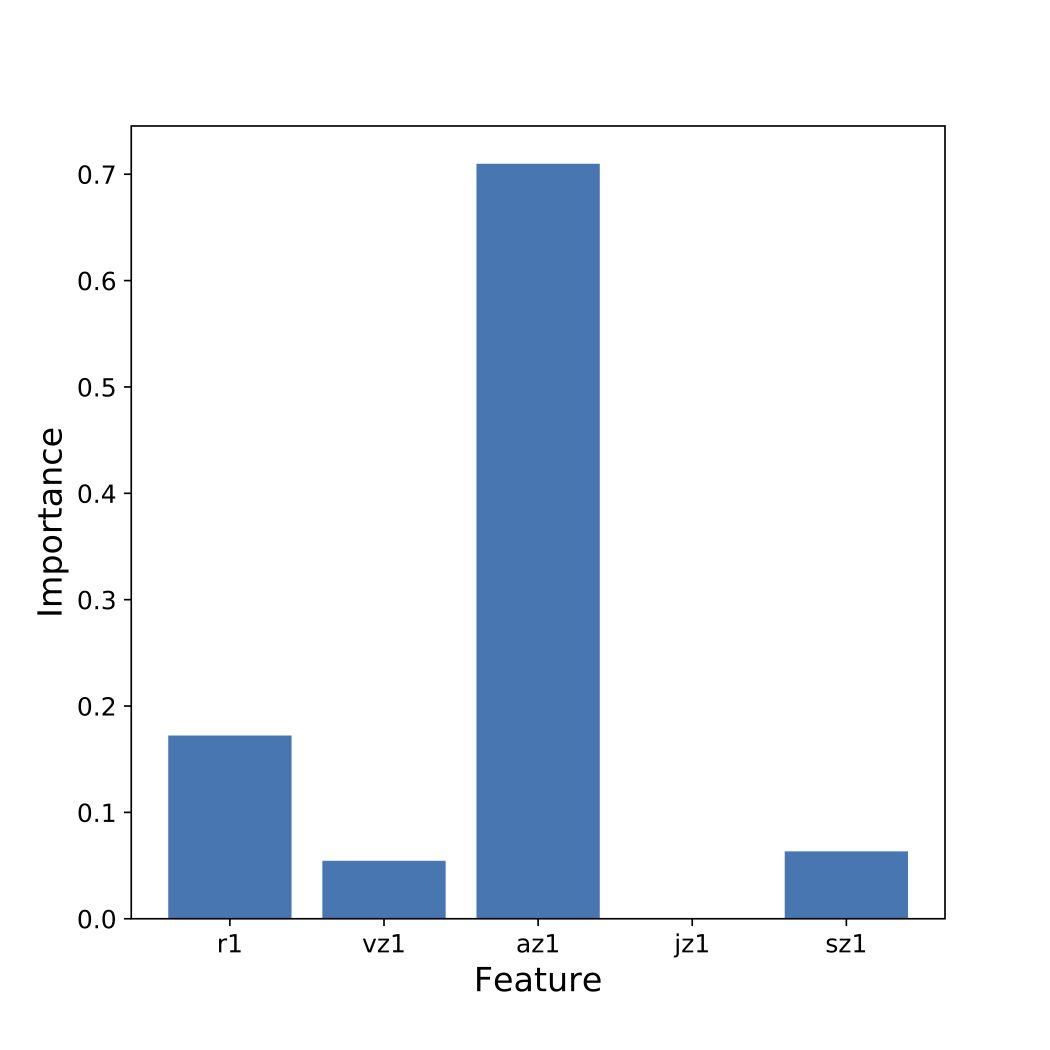
\includegraphics[width = 3in]{images/bar_imp_1part.png}}\\

\subfloat[5 MSPs per ammasso.]{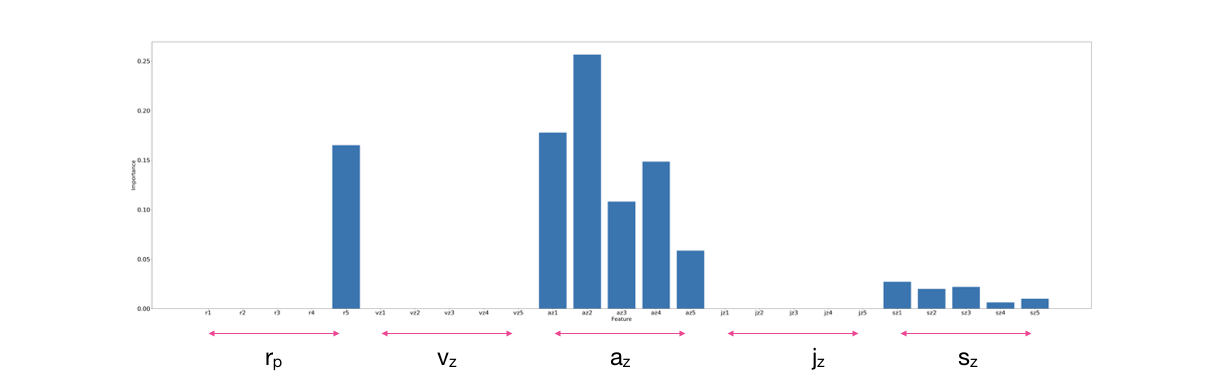
\includegraphics[width = 6in]{images/bar_imp_5part.png}}\\

\subfloat[10 MSPs per ammasso.]{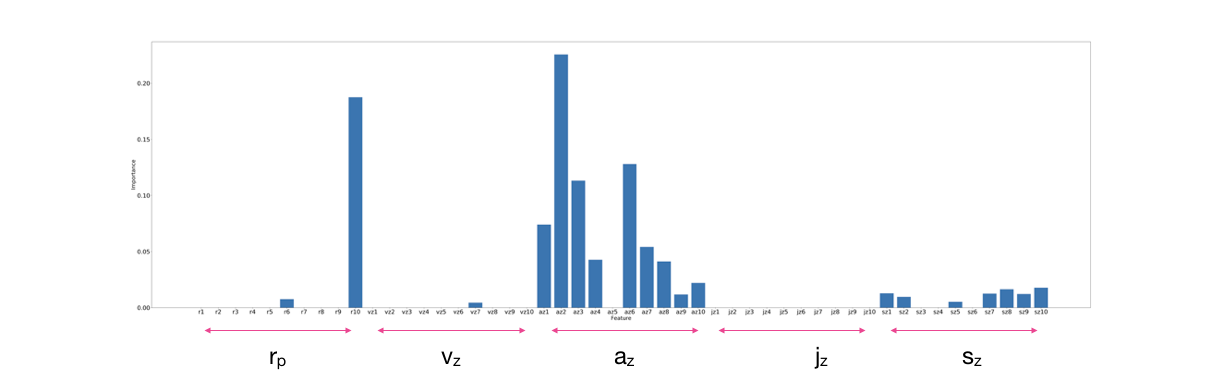
\includegraphics[width = 6in]{images/bar_imp_10part.png}}
\caption{Grafici delle importanze delle \textit{features} per il modello calcolate per i \textit{dataset} relativi a 1, 5 e 10 MSPs per ammasso (dall'alto verso il basso).}
\label{fig:importanze}
\end{figure}

\begin{figure}[H]
\centering
\subfloat[20 MSPs per ammasso.]{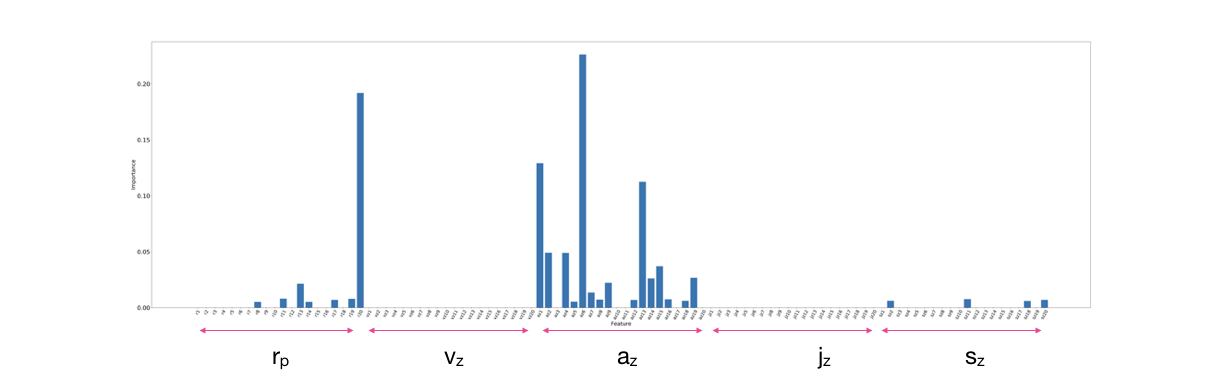
\includegraphics[width = 6in]{images/bar_imp_20part.png}}\\

\subfloat[30 MSPs per ammasso.]{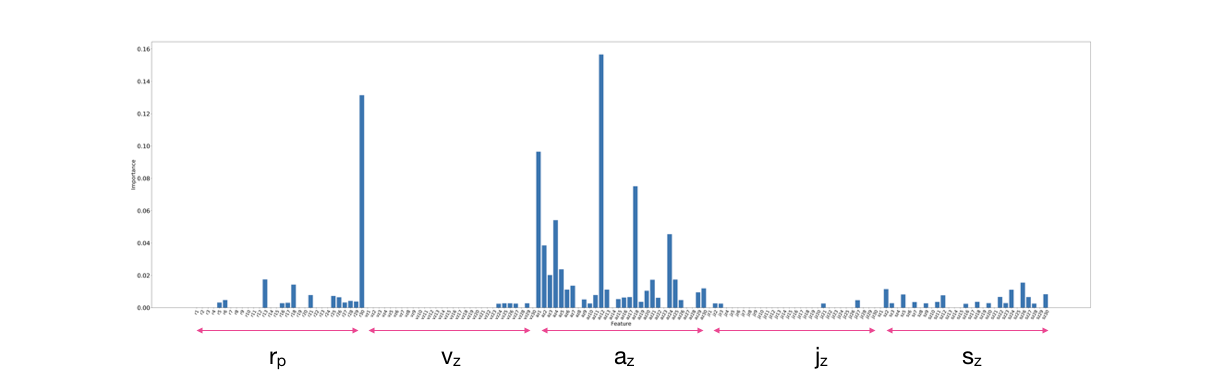
\includegraphics[width = 6in]{images/bar_imp_30part.png}}\\

\subfloat[40 MSPs per ammasso.]{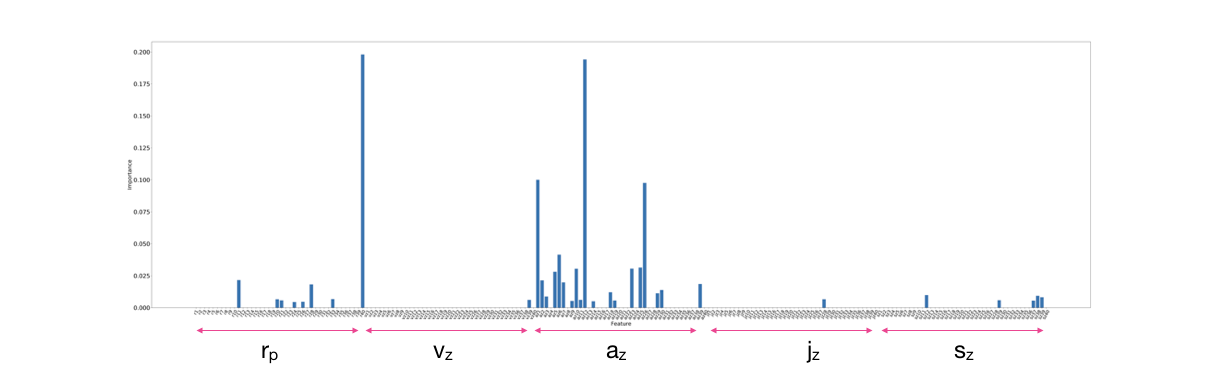
\includegraphics[width = 6in]{images/bar_imp_40part.png}}
\caption{Grafici delle importanze delle \textit{features} per il modello calcolate per i \textit{dataset} relativi a 20, 30 e 40 MSPs per ammasso (dall'alto verso il basso).}
\label{fig:importanze1}
\end{figure}


